\chapter{Introducción específica} % Main chapter title

\label{Chapter2}

%----------------------------------------------------------------------------------------
%	SECTION 1
%----------------------------------------------------------------------------------------
En el presente capítulo se describen los componentes de hardware, software, protocolos de comunicación y plataformas IoT utilizados para realizar el trabajo.

\section{Componentes principales de hardware}
\label{sec:ejemplo}

\subsection{Plataforma de desarrollo STM32 NUCLEO-L432KC}
La placa STM32 Nucleo-L432KC que se muestra en la figura \ref{fig:nucleol432kc} proporciona una forma asequible y flexible para que los usuarios prueben nuevos conceptos y construyan prototipos eligiendo entre las diversas combinaciones de funciones de rendimiento y consumo de energía que proporciona el microcontrolador STM32L4KC \citep{NUCLEOL432KC}.
\\ 
\\ Características:
\begin{itemize}
	\item Microcontrolador STM32L4KC en paquete 32 de pines.
	\item Led de usuario.
	\item Pulsador de reset.
	\item Conector de expansión Arduino Nano V3.
	\item Conector USB Micro-AB para ST-LINK.
	\item Opciones flexibles de fuente de alimentación.
	\item Depurador/programador ST-LINK integrado.
	\item Compatibilidad con una amplia variedad de entornos de desarrollo integrado.
	\item Oscilador de cristal de 24 MHz.
	\item Compatible con Arm Mbed Enabled.   
\end{itemize}
\begin{figure}[htbp]
	\centering
	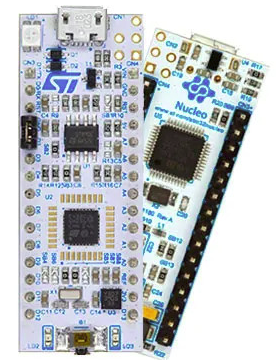
\includegraphics[width=4cm, height=5cm]{./Figures/nucleo-l432kc.png}
	\caption{Plataforma de desarrollo NUCLEO-L432KC\protect\footnotemark.}
	\label{fig:nucleol432kc}
\end{figure}
\vspace{5cm}
\footnotetext[1]{Datasheet \url{https://www.st.com/resource/en/user_manual/um1956-stm32-nucleo32-boards-mb1180-stmicroelectronics.pdf}}
\subsection{Módulo de comunicación LTE IOT 2 CLICK}
\label{subsec:ejemplo}
LTE IoT 2 click que se muestra en la \ref{fig:modulo LTE IOT} está equipado con el módulo BG96 LTE de Quectel Wireless Solutions, que admite tecnologías LTE CAT M1 y NB1, desarrolladas para aplicaciones IoT. Además, admite EGPRS a 850/900/1800/1900 MHz, lo que significa que se puede usar globalmente; no está restringido a ninguna región \citep{MonuloLTE-IOT}.
\\ 
\\Características:
\begin{itemize}
	\item Protocolos de internet integrados (TCP/UDP/PPP).
	\item Conectores SMA integrados.
	\item Leds de alimentación e indicación de estado.
	\item Conector USB para conectarlo con la aplicación de software de Quectel.
	\item Interfaz UART. 
	\item Tensión de alimentación 5 V o 3,3 V.
\end{itemize}
\begin{figure}[htbp]
	\centering
	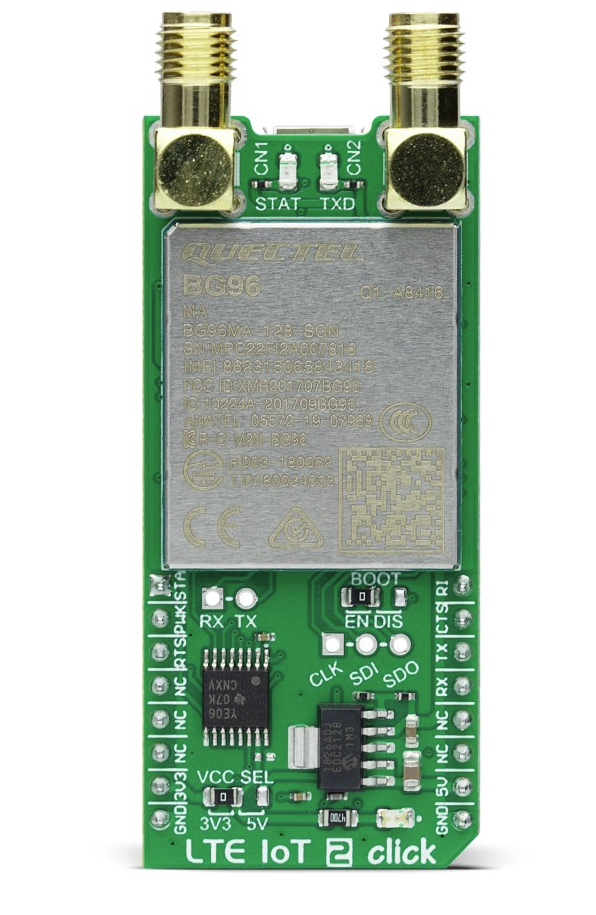
\includegraphics[width=4cm, height=5.5cm]{./Figures/moduloBG96.png}
	\caption{Módulo LTE IOT 2 CLICK\protect\footnotemark.}
	\label{fig:modulo LTE IOT}
\end{figure}

\footnotetext[2]{Imagen tomada de la página \url{https://www.mikroe.com/lte-iot-2-click}}
\subsection{Sensor AHT10}
El sensor AHT10 presentado en la figura \ref{fig:SensorAHT10} permite obtener lecturas de temperatura y humedad, es de bajo costo y excelente rendimiento. Se utiliza este sensor en aplicaciones de control automático de temperatura, aire acondicionado, estaciones meteorológicas, aplicaciones en el hogar, regulador de humedad y temperatura \citep{ModuloAHT10}.
\begin{figure}[htbp]
	\centering
	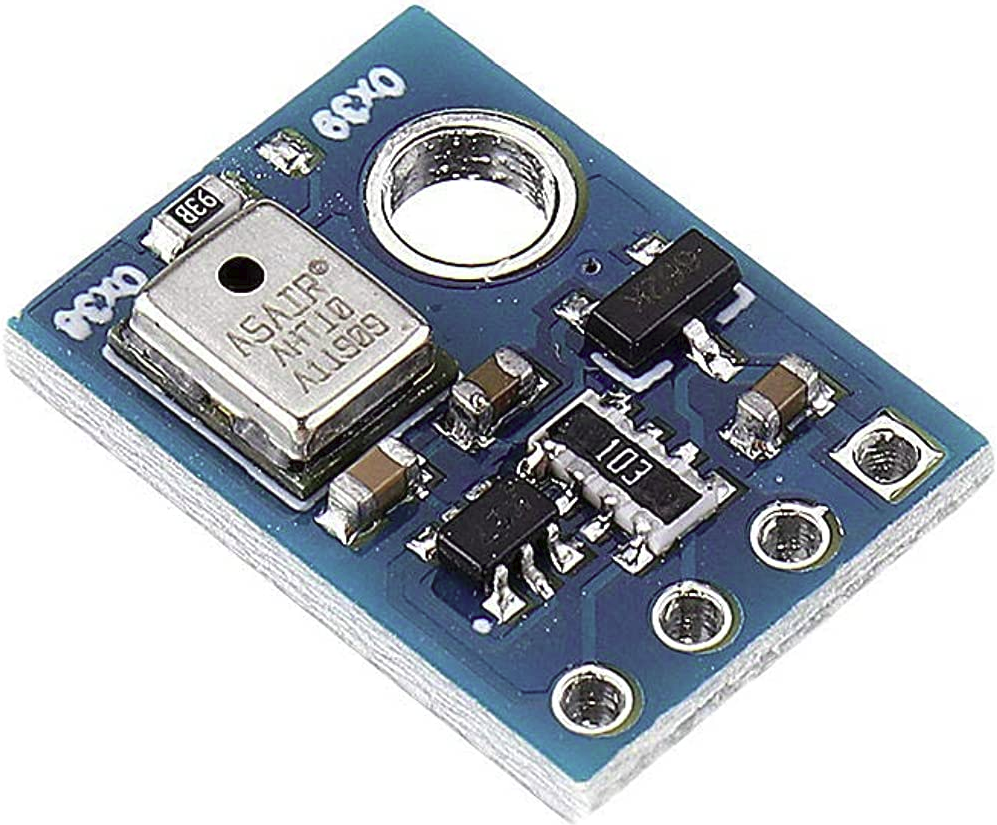
\includegraphics[width=.3\textwidth]{./Figures/aht10.png}
	\caption{Sensor AHT10\protect\footnotemark.}
	\label{fig:SensorAHT10}
\end{figure}
\footnotetext[3]{Imagen tomada de la página \url{https://esphome.io/components/sensor/aht10.html}}
\subsection{Sensor ML8511}
El módulo ML8511 presentado en la figura \ref{fig:SensorML8511} es un sensor de luz ultravioleta (UV), entrega una señal de tensión analógica que depende de la cantidad de luz UV que detecta. Sensor ideal para proyectos de monitoreo de condiciones ambientales como el índice UV, aplicaciones meteorológicas, cuidado de la piel, medición industrial de nivel UV.
El sensor ML8511 detecta luz con una longitud de onda entre 280-390 nm, este rango cubre tanto al espectro UV-B como al UV-A. La salida analógica está relacionada linealmente con la intensidad UV $(mW/cm^2)$ \citep{ModuloML8511}.
\begin{figure}[htbp]
	\centering
	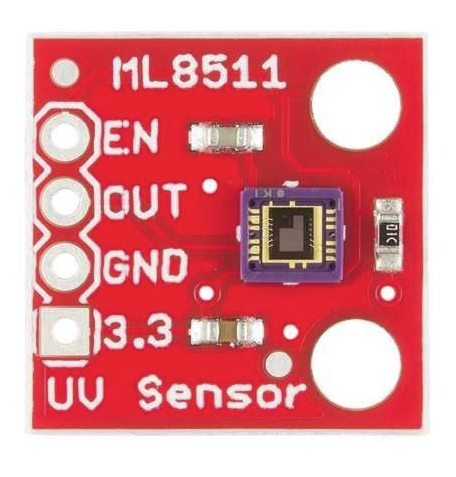
\includegraphics[width=.3\textwidth]{./Figures/ml8511.png}
	\caption[Módulo Sensor ML8511]{Módulo Sensor ML8511. \footnotemark }
	\label{fig:SensorML8511}
\end{figure}


\footnotetext[4]{Manual del sensor \url{https://learn.sparkfun.com/tutorials/ml8511-uv-sensor-hookup-guide/all}}
\subsection{Sensor de humedad de suelo HL-69 (Resistivo)}
El módulo HL-69 presentado en la figura \ref{fig:SensorHL-69}, un sensor de humedad de suelo que utiliza la conductividad entre dos terminales para determinar parámetros relacionados al agua, líquidos y humedad \citep{ModuloHL-69}.
\begin{figure}[htbp]
	\centering
	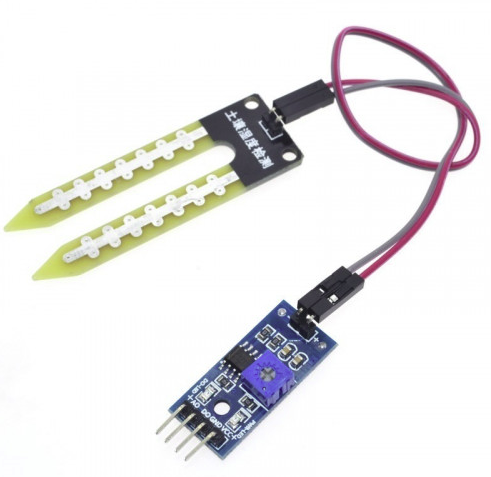
\includegraphics[width=4.5cm, height=4.5cm]{./Figures/sensordehumedad.png}
	\caption{Módulo sensor HL-69\protect\footnotemark.}
	\label{fig:SensorHL-69}
\end{figure}

\section{Herramientas de software y testing utilizados}
\subsection{STM32 CubeIDE}
STM32CubeIDE es una herramienta de desarrollo multi-OS todo en uno, que forma parte del ecosistema de software STM32Cube. Se trata de una plataforma de desarrollo C/C++ que permite compilar y depurar código para los microcontroladores STM32. Se basa en el marco Eclipse  y la cadena de herramientas GCC para el desarrollo y GDB para la depuración. Permite la integración de los cientos de plugins existentes que completan las funcionalidades del IDE de Eclipse \citep{STM32CUBEIDE}.

Integra las funcionalidades de configuración y creación de proyectos de STM32 de STM32CubeMX para ofrecer una experiencia de herramienta todo en uno y ahorrar tiempo de instalación y desarrollo \citep{STM32CUBEIDE}.

\subsection{FreeRTOS}
\label{subsec:FreeRTOS}
FreeRTOS es un sistema operativo en tiempo real (RTOS) líder en el mercado para microcontroladores y pequeños microprocesadores. Distribuido libremente bajo la licencia de código abierto del MIT, FreeRTOS incluye un núcleo y un conjunto creciente de bibliotecas adecuadas para su uso en todos los sectores de la industria.
FreeRTOS está diseñado con énfasis en la confiabilidad, la accesibilidad y la facilidad de uso \citep{FreeRTOS}. El logo de FreeRTOS se muestra en la figura \ref{fig:FreeRTOS}.
\begin{figure}[htbp]
	\centering
	
\includegraphics[width=6cm, height=2cm]{./Figures/logo_FreeRTOS.png}
	\caption{Logo FreeRTOS\protect\footnotemark.}
	\label{fig:FreeRTOS}
\end{figure}
\footnotetext[5]{Tienda \url{https://tienda.sawers.com.bo/hl-69-modulo-sensor-humedad-suelo}}
\footnotetext[6]{Imagen tomada de la página \url{https://www.freertos.org/}}
\subsection{CEEDLING}
Ceedling es un sistema de compilación diseñado para proyectos en lenguaje C, que podría describirse como una extensión del sistema de compilación Rake (similar a make) de Ruby. Ceedling está dirigido principalmente al desarrollo basado en pruebas en C y está diseñado para reunir CMock, Unity y CException \citep{CEEDLING}.

\section{Protocolos de Comunicación}
\subsection{UART}
UART (\textit{Universal Asynchronous Receiver / transmitter}, por sus siglas en inglés) define un protocolo o un conjunto de normas para el intercambio de datos en serie entre dos dispositivos. UART es sumamente simple y utiliza solo dos hilos entre el transmisor y el receptor para transmitir y recibir en ambas direcciones. Ambos extremos tienen una conexión a masa. La comunicación en UART puede ser simplex (los datos se envían en una sola dirección), semidúplex (cada extremo se comunica, pero solo uno al mismo tiempo), o dúplex completo (ambos extremos pueden transmitir simultáneamente). Los datos se transmiten en forma de tramas \citep{UART}.
\subsection{I2C}

El protocolo I2C (\textit {Inter-Integrated Circuit}) es un protocolo diseñado para permitir la comunicación entre múltiples circuitos integrados digitales y uno o más chips controladores. Similar a la interfaz periférica en serie, está destinado a comunicaciones de corta distancia dentro de un solo dispositivo. Al igual que las interfaces seriales asíncronas, solo requiere dos cables de señal para el intercambio de información \citep{I2C}.

\subsection{MQTT}
MQTT es un protocolo de mensajería estándar de OASIS para IoT. Está diseñado como un transporte de mensajería de publicación/suscripción extremadamente liviano que es ideal para conectar dispositivos remotos con un espacio de código pequeño y un ancho de banda de red mínimo. MQTT hoy en día se utiliza en una amplia variedad de industrias, como la automotriz, la manufactura, las telecomunicaciones, el petróleo y el gas, etc \citep{MQTT}. En la figura \ref{fig:ArquitecturaMQTT} se muestra la arquitectura del protocolo MQTT.
\footnotetext[7]{Imagen tomada de la página \url{https://mqtt.org/}}
\begin{figure}[htbp]
	\centering
	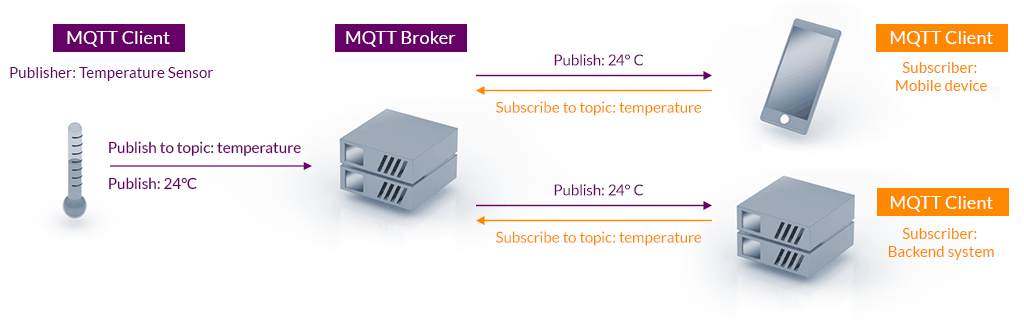
\includegraphics[width=\textwidth, height=3.3cm]{./Figures/mqtt-publish-subscribe.png}
	\caption{Arquitectura de publicación/suscripción de MQTT\protect\footnotemark.}
	\label{fig:ArquitecturaMQTT}
\end{figure}

\section{Plataformas IoT}
\subsection{Ubidots}
Ubidots permite enviar datos de sensores a la nube, configurar tableros y alertas, conectarse con otras plataformas, usar herramientas de analítica y arrojar mapas de datos en tiempo real \citep{InterfazIoTUbidots}. En la figura \ref{fig:InterfazUBIDOTS} se muestra un ejemplo de interfaz gráfica en Ubidots.
\footnotetext[8]{Imagen tomada de la página \url{https://ubidots.com/platform/time-series}}
\footnotetext[9]{Imagen tomada de la página \url{https://thingsboard.io/smart-farming/}}

\begin{figure}[htbp]
	\centering
	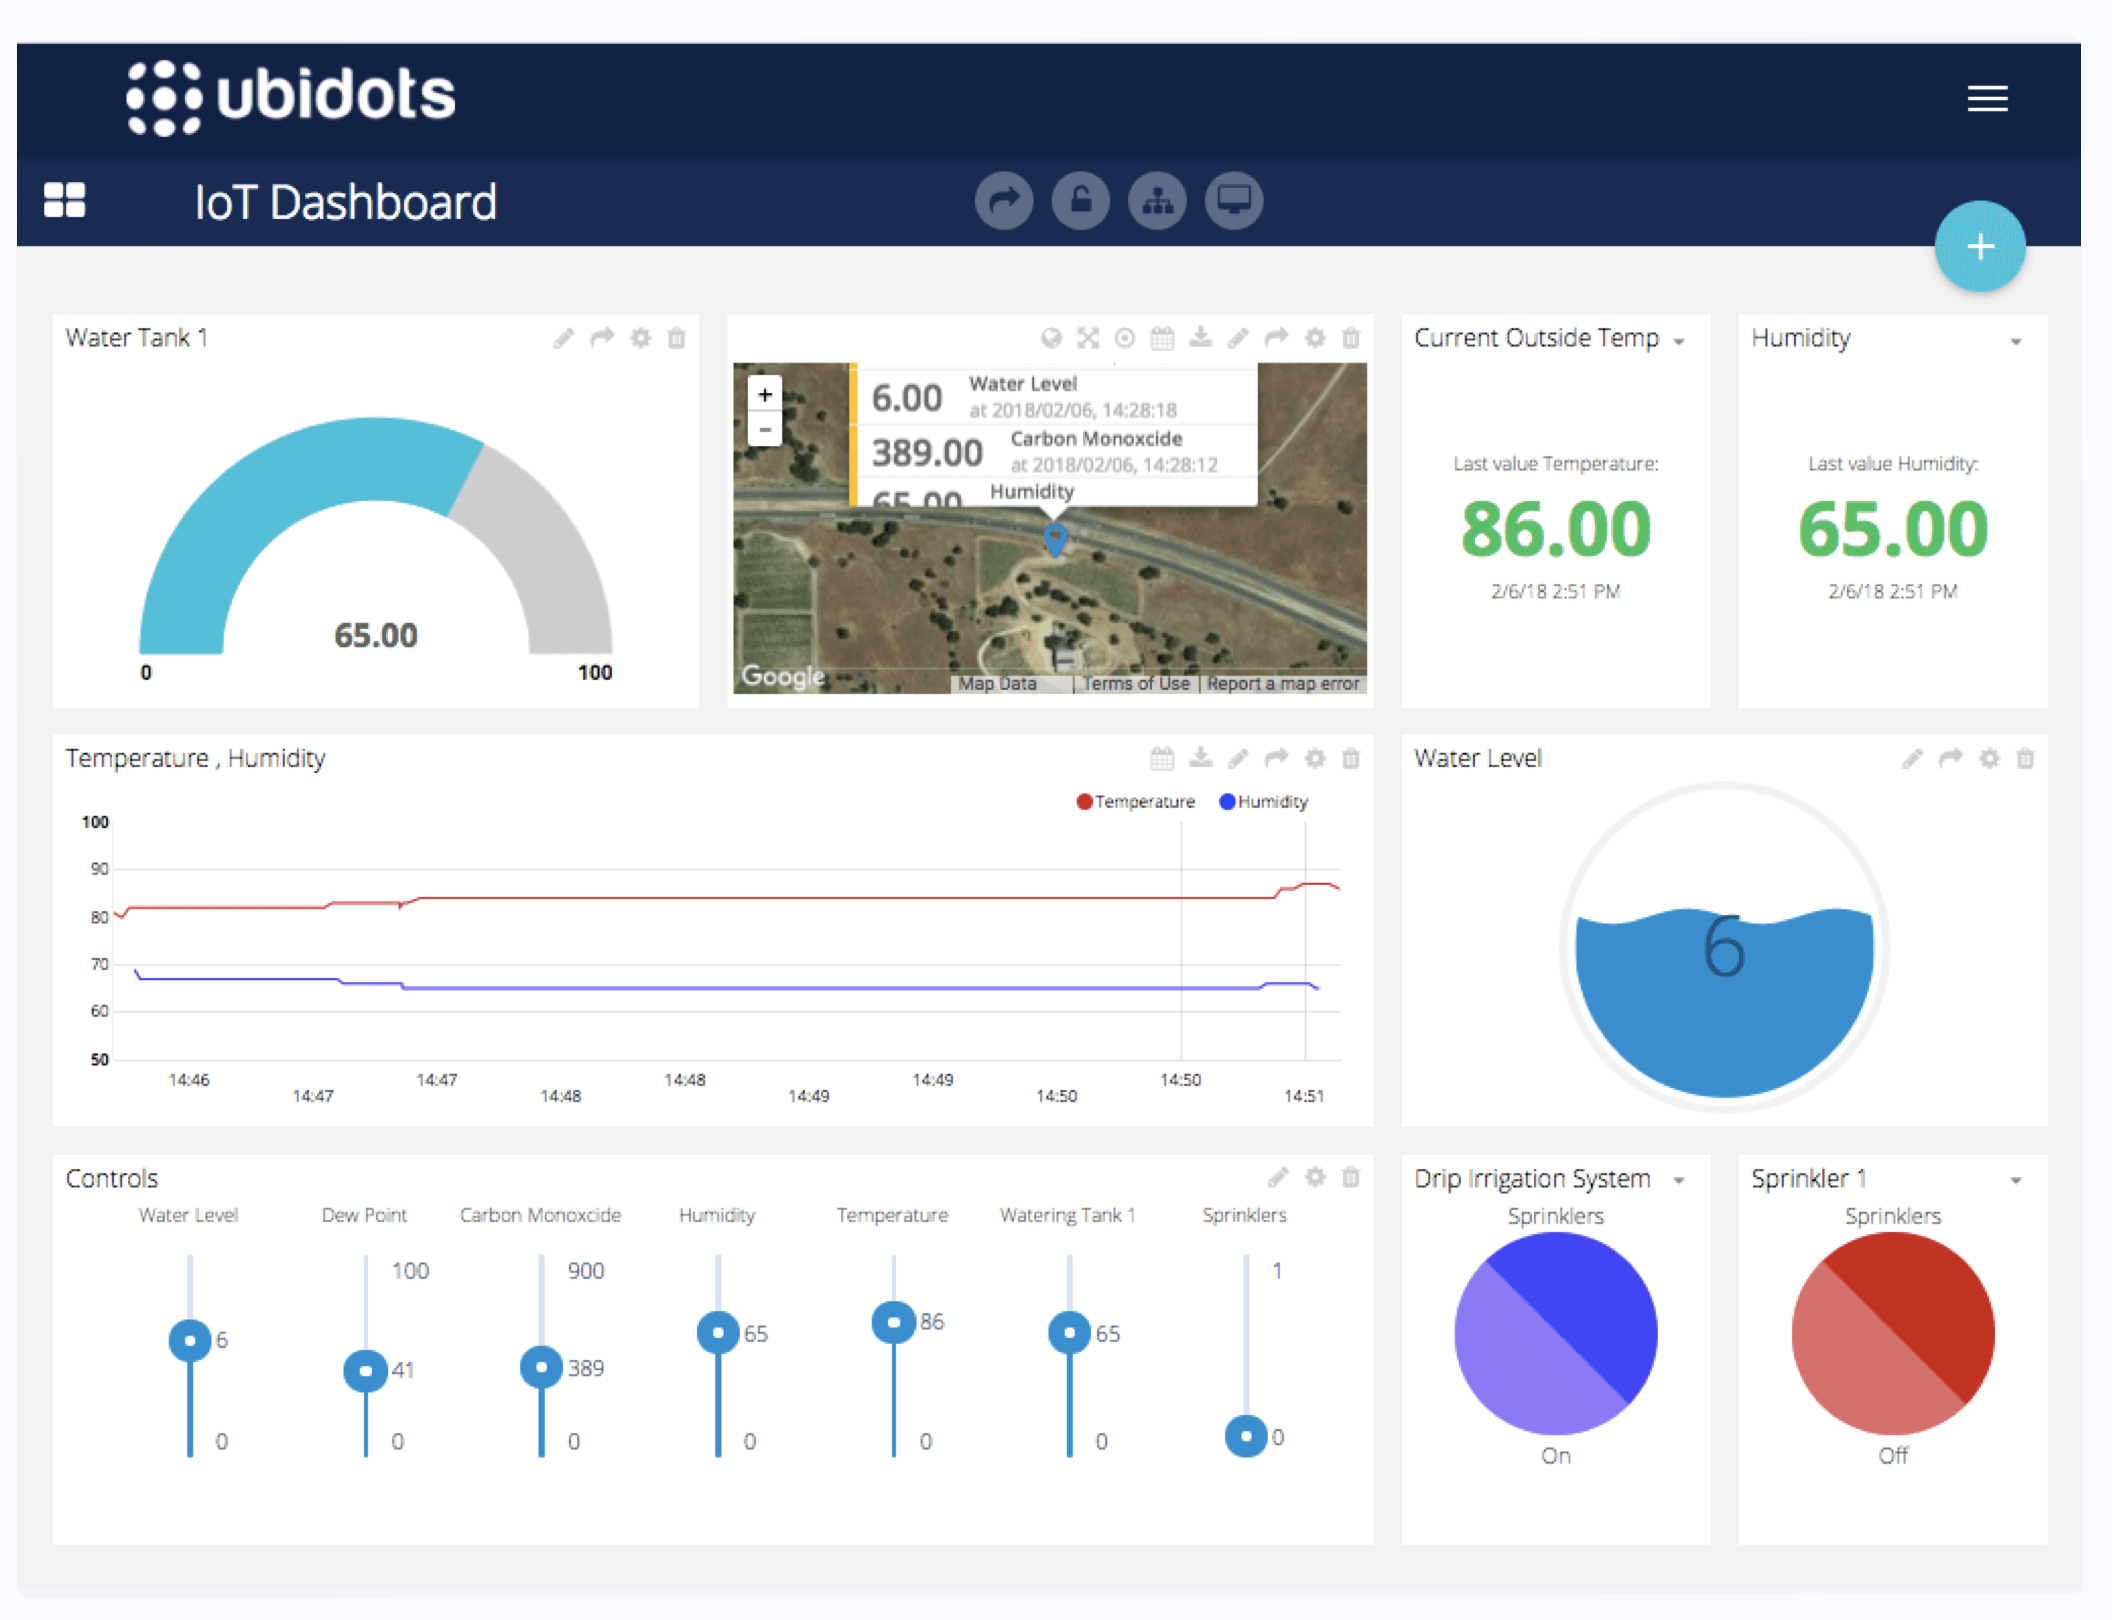
\includegraphics[width=10cm, height=6cm]{./Figures/ubidots.png}
	\caption{Ejemplo interfaz gráfica Ubidots\protect\footnotemark.}
	\label{fig:InterfazUBIDOTS}
\end{figure}
\subsection{ThingsBoard}
ThingsBoard es una plataforma IoT de código abierto para la recopilación, el procesamiento, la visualización y la gestión de dispositivos.
Permite la conectividad de dispositivos a través de protocolos estándares de la industria IoT: MQTT, CoAP y HTTP. ThingsBoard combina escalabilidad, tolerancia a fallas y rendimiento \citep{THINGSBOARD}. En la figura \ref{fig:InterfazThingsBoard} se muestra un ejemplo de una interfaz gráfica desarrollada en ThingsBoard. 

\begin{figure}[htbp]
	\centering
	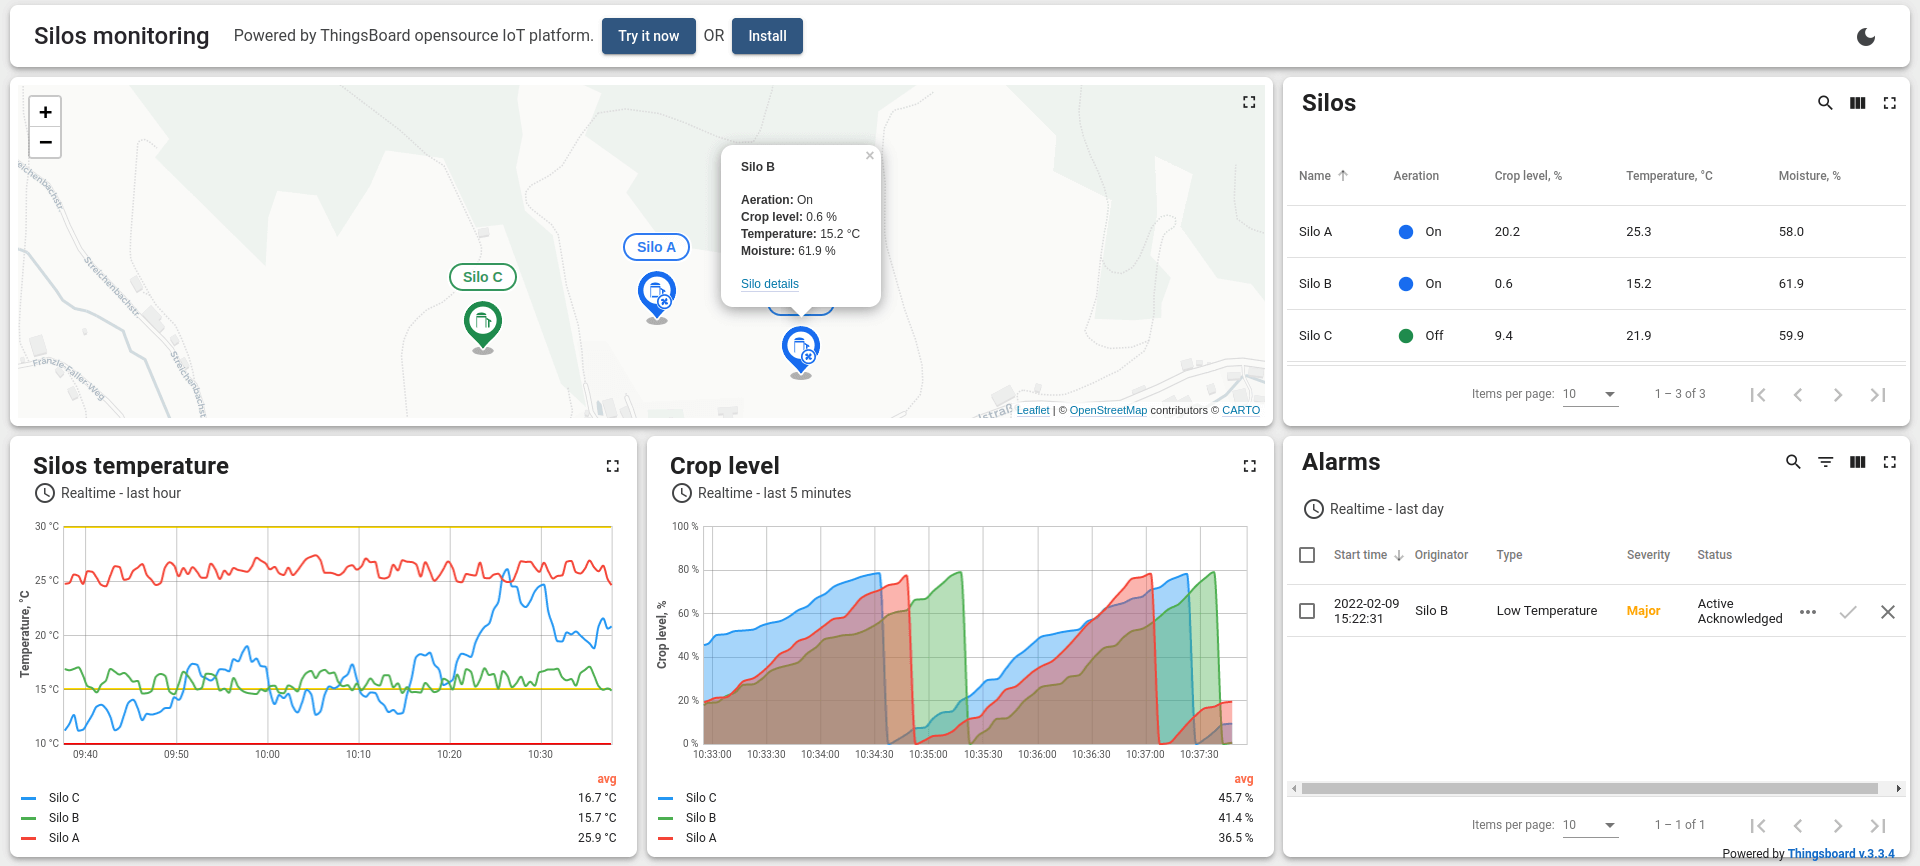
\includegraphics[width=10cm, height=5.5cm]{./Figures/thingsboard.png}
	\caption{Ejemplo interfaz gráfica ThingsBoard\protect\footnotemark.}
	\label{fig:InterfazThingsBoard}
\end{figure}